\subsection{Programming GPs pt. 2}

The code can be found in~\cref{sec:week5:code:exercise}.

The posterior distribution $p(f^\ast | u, S \cup x^\ast)$
using the \emph{Gaussian} kernel is shown in~\cref{fig:week5:gp:predict:gauss}.
The noise variance was chosen to be $\sigma_y = 0.005$
and the single parameter was chosen to be $\gamma = 11.555\ldots$,
both by performing grid-search on
${ (\sigma_y, \gamma) \in [0.005, 1] \times [1, 20] }$.
%
As can be seen, the prediction is very poor,
and it has a large area of uncertainty.
Despite the large area of uncertainty,
$\sim\!74\%$ of the test points lie outside
the 95\% uncertainty area, and the model has an
$R^2$ score of $\sim\!-7.5$ indicating that the Gaussian kernel is the wrong model
for predicting this data.

The posterior distribution
using the \emph{special} kernel is shown in~\cref{fig:week5:gp:predict:special}.
The noise variance was chosen to be $\sigma_y = 0.11555\ldots$
and the parameters were chosen to be $a = 1.112$, $b = 8.889$,
both by performing grid-search on
${ (\sigma_y, a, b) \in [0.005, 1] \times [0.001, 10] \times [0.001, 10] }$.
%
From the plot, we see that this prediction follows the shape of the test data,
and also has a much smaller unceartainty, which indicates that it is a better
fit for the data than the Gaussian kernel.
This is also evident as $\sim\!49\%$ of the test points lie outside the
95\% unceartainty area, and an $R^2$ score of $\sim\!0.61$.
While these metrics are not great, they are much better than
the ones for the Gaussian kernel.

\begin{figure}[htbp]
  \centering
  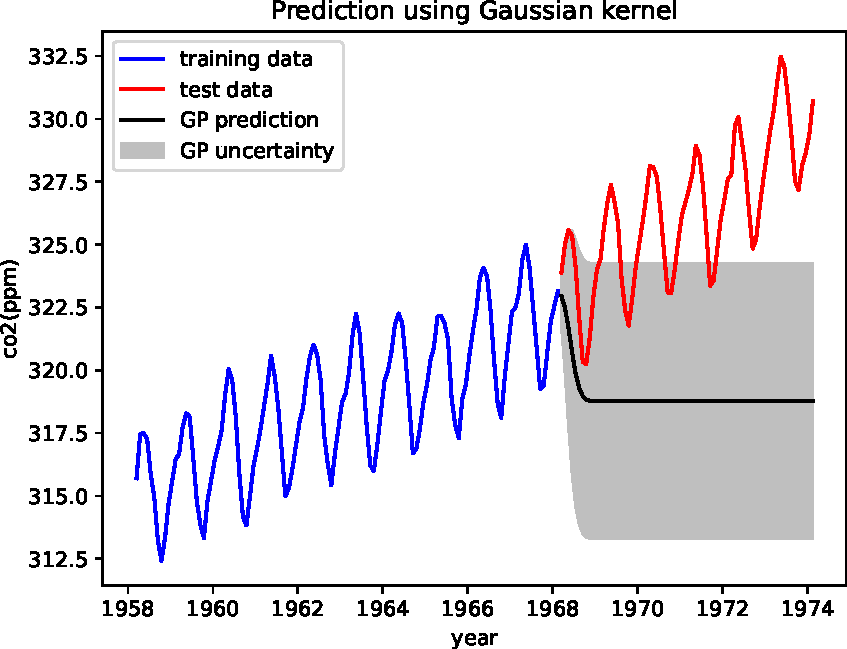
\includegraphics[width=0.7\textwidth]{./figures/gp_predict_gaussian.pdf}
  \caption{
    Posterior of Gaussian kernel trained on
    CO2 measurements at Mauna Loa, Hawaii.
  }
  \label{fig:week5:gp:predict:gauss}
\end{figure}

\begin{figure}[htbp]
  \centering
  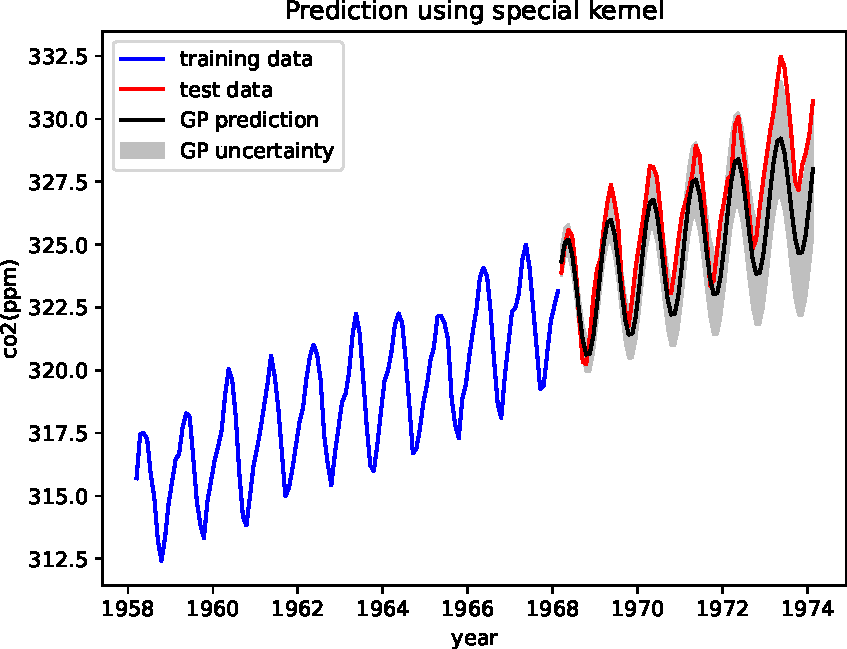
\includegraphics[width=0.7\textwidth]{./figures/gp_predict_special.pdf}
  \caption{
    Posterior of special kernel trained on
    CO2 measurements at Mauna Loa, Hawaii.
  }
  \label{fig:week5:gp:predict:special}
\end{figure}
